\documentclass[conference]{IEEEtran}
\IEEEoverridecommandlockouts

\usepackage{cite}
\usepackage{amsmath,amssymb,amsfonts}
\usepackage{algorithmic}
\usepackage{graphicx}
\usepackage{textcomp}
\usepackage{xcolor}
\usepackage{array}
\usepackage{booktabs}
\usepackage{multirow}
\usepackage{tikz}
\usetikzlibrary{arrows.meta,positioning,shapes.geometric}

\begin{document}

\title{Hardware-Efficient Spiking Neural Networks using Dynamic Gatekeeping and Early Exit Control\\
\thanks{Project report submitted for ECE 274: Neuromorphic Computing, Winter 2025.}
}

\author{
\IEEEauthorblockN{Siddhesh Uttarwar}
\IEEEauthorblockA{\textit{Department of Electrical and Computer Engineering} \\
\textit{University of California, Santa Barbara}\\
Santa Barbara, CA, USA \\
Email: suttarwa@ucsb.edu}
\and
\IEEEauthorblockN{Parth Kulkarni}
\IEEEauthorblockA{\textit{Department of Electrical and Computer Engineering} \\
\textit{University of California, Santa Barbara}\\
Santa Barbara, CA, USA \\
Email: parthkulkarni@ucsb.edu}
}

\maketitle

% ============================================================
% ABSTRACT
% ============================================================
\begin{abstract}
Spiking Neural Networks (SNNs) are attractive for edge inference due to their event-driven sparsity, yet practical energy savings are often limited by memory traffic and fixed-latency execution. This paper presents a hardware-software co-designed convolutional SNN (CSNN) inference pipeline that combines three orthogonal optimizations: (i) a dynamic gatekeeper that suppresses low-information and redundant spike events before any memory access, (ii) adaptive LIF thresholding per neuron to enforce temporal sparsity, and (iii) a confidence-driven early exit controller that terminates inference once classification certainty is reached. Each optimization is simultaneously expressed in PyTorch (for training and validation) and as synthesizable Verilog RTL (for hardware deployment). Evaluated over 500 test samples on N-MNIST with INT8-quantized weights, the proposed sparse design achieves 90.8\% accuracy (vs. 97.6\% baseline), reduces average SRAM reads from 70,824 to 13,002 per inference (81.6\% reduction), and lowers estimated inference energy from 368~pJ to 68~pJ based on published 45nm CMOS access costs. The gatekeeper independently rejects 23.9\% of input events, and early exit triggers at an average of $T$=11.4 instead of the full $T$=20 window. The complete hardware pipeline is functionally verified through Icarus Verilog simulation of synthesizable RTL modules. These results demonstrate that hardware-aware control logic can deliver substantial efficiency improvements beyond algorithmic sparsity alone, making the approach directly applicable to low-power neuromorphic edge accelerators.
\end{abstract}

\begin{IEEEkeywords}
Spiking Neural Networks, Neuromorphic Hardware, Event-Driven Computing, Dynamic Gatekeeping, Early Exit, N-MNIST, SRAM Efficiency, Software-Hardware Co-Design
\end{IEEEkeywords}

% ============================================================
% I. INTRODUCTION
% ============================================================
\section{Introduction}
Energy efficiency is the central constraint in deploying neural networks at the edge. While Spiking Neural Networks (SNNs) promise theoretical sparsity through event-driven computation, deployed systems still incur high cost when data movement and control are not explicitly co-designed with the model. In digital implementations running on CMOS, SRAM access dominates both power and latency budgets~\cite{horowitz2014energy}. According to published CMOS energy data~\cite{horowitz2014energy}, a single 8-bit SRAM read at 45nm costs approximately 5~pJ---170$\times$ more energy than an integer addition---making memory traffic the primary optimization target in any digital SNN accelerator.

Prior work on SNNs has focused on algorithmic improvements such as surrogate gradient training~\cite{neftci2019surrogate}, temporal coding~\cite{zenke2021remarkable}, and threshold adaptation~\cite{bellec2018long}. However, these approaches rarely quantify their impact on hardware-level metrics like SRAM read counts, memory-port utilization, or inference latency in clock cycles. As a result, the connection between ``sparse model'' and ``energy-efficient hardware'' remains qualitative.

This project bridges that gap through a \textbf{hardware-first design objective}: reduce memory-read activity without sacrificing useful classification accuracy. We start from a surrogate-gradient-trained LeNet-5 CSNN baseline and introduce three architectural controls:
\begin{itemize}
    \item \textbf{Dynamic gatekeeping:} An input-side filter that prevents low-value and redundant spikes from triggering downstream memory reads, implemented as a combinational event classifier with saturating counters and burst detection.
    \item \textbf{Adaptive threshold regulation:} A per-neuron threshold that increases after firing and decays over time, suppressing spike storms and enforcing temporal sparsity across all hidden layers.
    \item \textbf{Confidence-driven early exit:} An output-side FSM that monitors classification confidence and globally halts the inference pipeline once a decision threshold is crossed.
\end{itemize}

Critically, each mechanism is simultaneously implemented in PyTorch (for gradient-based training and large-scale evaluation) and in synthesizable Verilog RTL (for hardware deployment), ensuring that software-level accuracy and hardware-level efficiency are validated against the same dataflow. The full Verilog module set is provided in the repository, and hardware-proxy counters in the PyTorch forward pass produce metrics that map directly to RTL control signals.

% ============================================================
% II. DATASET AND PREPROCESSING
% ============================================================
\section{Dataset and Preprocessing Pipeline}

\subsection{N-MNIST Event Stream}
N-MNIST converts static MNIST digits into asynchronous event streams captured by a Dynamic Vision Sensor (DVS) under controlled saccadic motion~\cite{orchard2015converting}. Each event is a tuple $(x, y, p, t)$ comprising pixel coordinates, polarity (ON/OFF), and a microsecond-resolution timestamp. The dataset contains 60,000 training and 10,000 test samples across 10 digit classes.

\subsection{Spatial Normalization}
The native sensor resolution of $34\times34$ pixels is center-cropped to $28\times28$ to align with the LeNet-5 convolutional kernel sizes:
\begin{equation}
x' = x - 3, \quad y' = y - 3.
\end{equation}
Events outside the retained 28$\times$28 region are discarded as peripheral noise from the saccadic motion.

\subsection{Temporal Binning}
Continuous timestamps are discretized into $T=20$ uniform time bins across the $\sim$300~ms recording horizon:
\begin{equation}
b_i = \text{clip}\!\left(\left\lfloor \frac{t_i - t_{\min}}{t_{\max} - t_{\min}} \cdot T \right\rfloor, 0, T{-}1\right).
\end{equation}
Polarity channels are preserved, yielding input spike tensors of shape $(T, 2, 28, 28)$. This representation maintains temporal structure while enabling batched training and hardware-style stepwise execution.

\begin{figure}[htbp]
\centerline{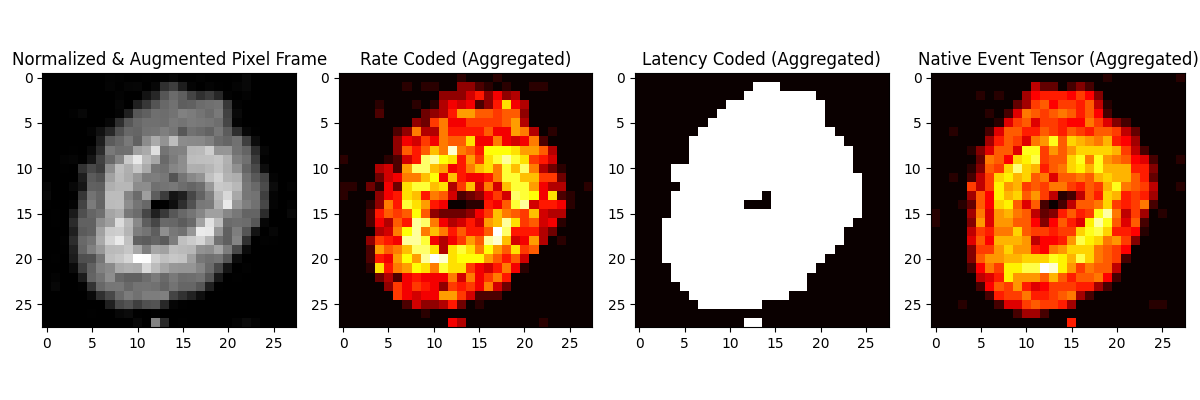
\includegraphics[width=\linewidth]{plots/preprocessing_pipeline.png}}
\caption{Preprocessing flow: raw AER events $\rightarrow$ spatial cropping $\rightarrow$ temporal binning $\rightarrow$ binary spike tensors.}
\label{fig:preprocessing}
\end{figure}

% ============================================================
% III. MODEL AND LEARNING METHOD
% ============================================================
\section{Model Architecture and Training}

\subsection{CSNN Topology}
The baseline network follows a modified LeNet-5 topology adapted for event-based data and spiking neurons. The full structural details are given in Table~\ref{tab:lenet_struct}. Key modifications from the original LeNet-5 include: 2-channel polarity input, Leaky Integrate-and-Fire (LIF) neurons replacing ReLU activations, average pooling instead of max pooling (to preserve spike firing density), and batch normalization before each LIF layer.

\begin{table*}[t]
\caption{LeNet-5 Sparse CSNN -- Layer Configuration (Per Timestep, Shared Weights)}
\centering
\scriptsize
\setlength{\tabcolsep}{3.2pt}
\resizebox{\textwidth}{!}{%
\begin{tabular}{|c c c|c c c|c|c|c|c c|c|c|c|}
\hline
\multicolumn{3}{|c|}{\textbf{Input}} & \multicolumn{3}{c|}{\textbf{Output}} & \textbf{Layer} & \textbf{Stride} & \textbf{Pad} & \multicolumn{2}{c|}{\textbf{Kernel}} & \textbf{in} & \textbf{out} & \textbf{\# Param} \\
\hline
\textbf{H} & \textbf{W} & \textbf{C} & \textbf{H} & \textbf{W} & \textbf{C} & & & & \textbf{H} & \textbf{W} & & & \\
\hline
28 & 28 & 2 & 28 & 28 & 32 & conv1    & 1 & 2 & 5 & 5 & 2    & 32  & 1,600   \\
28 & 28 & 32 & 28 & 28 & 32 & bn1      & - & - & - & - & 32   & 32  & 64      \\
28 & 28 & 32 & 28 & 28 & 32 & lif1     & 1 & - & - & - & 32   & 32  & 0       \\
28 & 28 & 32 & 14 & 14 & 32 & avgpool1 & 2 & 0 & 2 & 2 & 32   & 32  & 0       \\
14 & 14 & 32 & 14 & 14 & 64 & conv2    & 1 & 2 & 5 & 5 & 32   & 64  & 51,200  \\
14 & 14 & 64 & 14 & 14 & 64 & bn2      & - & - & - & - & 64   & 64  & 128     \\
14 & 14 & 64 & 14 & 14 & 64 & lif2     & 1 & - & - & - & 64   & 64  & 0       \\
14 & 14 & 64 & 7  & 7  & 64 & avgpool2 & 2 & 0 & 2 & 2 & 64   & 64  & 0       \\
7  & 7  & 64 & 1  & 1  & 3136 & flatten & - & - & - & - & 3136 & 3136 & 0    \\
1  & 1  & 3136 & 1  & 1  & 3136 & dropout & - & - & - & - & 3136 & 3136 & 0 \\
1  & 1  & 3136 & 1  & 1  & 128 & fc1     & - & - & 1 & 1 & 3136 & 128 & 401,408 \\
1  & 1  & 128 & 1  & 1  & 128 & lif3     & 1 & - & - & - & 128  & 128 & 0       \\
1  & 1  & 128 & 1  & 1  & 10  & fc2      & - & - & 1 & 1 & 128  & 10  & 1,280   \\
1  & 1  & 10  & 1  & 1  & 10  & lif4     & 1 & - & - & - & 10   & 10  & 0       \\
\hline
\multicolumn{13}{|r|}{\textbf{Total Trainable Parameters}} & \textbf{455,680} \\
\hline
\multicolumn{14}{|l|}{\textit{Note: This block is reused across all $T$ time bins (weight sharing across time).}} \\
\hline
\end{tabular}
}
\label{tab:lenet_struct}
\normalsize
\end{table*}

\subsection{Leaky Integrate-and-Fire (LIF) Dynamics}
The membrane potential update at timestep $t$ is
\begin{equation}
V_j(t) = \beta \cdot V_j(t{-}1) + X_j(t),
\label{eq:lif}
\end{equation}
where $\beta=0.9$ is the leak factor, and $X_j(t)$ is the synaptic input current after batch normalization. Spiking follows a Heaviside threshold:
\begin{equation}
S_j(t) =
\begin{cases}
1, & V_j(t) \ge V_{th,j}(t) \\
0, & \text{otherwise.}
\end{cases}
\end{equation}
A soft-reset mechanism subtracts the threshold from membrane potential upon spiking, preserving residual charge:
\begin{equation}
V_j(t) \leftarrow V_j(t) - S_j(t) \cdot V_{th,j}(t).
\end{equation}

\subsection{Surrogate Gradient Training (STBP)}
Because the spike function is non-differentiable, backpropagation uses a fast-sigmoid surrogate derivative~\cite{neftci2019surrogate,zenke2021remarkable}:
\begin{equation}
\frac{\partial S}{\partial V} \approx \frac{1}{\left(1+\alpha|V-V_{th}|\right)^2},
\end{equation}
with $\alpha=2.0$. Training uses Adam optimizer with learning rate $10^{-3}$, cosine annealing schedule, and an L1 spike regularization loss to encourage overall sparsity:
\begin{equation}
\mathcal{L} = \mathcal{L}_{CE} + \lambda \sum_{t,\ell,j} S_j^{(\ell)}(t), \quad \lambda = 5 \times 10^{-4}.
\end{equation}

% ============================================================
% IV. HARDWARE-ORIENTED OPTIMIZATIONS
% ============================================================
\section{Hardware-Oriented Optimizations}

\subsection{Dynamic Gatekeeping}
A gatekeeper block is inserted ahead of Conv1 to evaluate each input spike event \textit{before} any memory access is issued. The gate combines two sub-circuits:

\subsubsection{Importance Monitor}
A 4-bit saturating counter array $I[c,y,x]$ tracks cumulative activity at each spatial position. Every $W{=}255$ clock cycles, all counters are decayed via hardware-efficient right-shift (divide-by-2). An event is classified as ``important'' if $I[\text{pre\_id}] \ge \theta_{\text{imp}}$ where $\theta_{\text{imp}}=1$, filtering noise that has not recurred at the same location.

\subsubsection{Burst Redundancy Filter}
A comparator tracks \texttt{last\_pre\_id} and a 3-bit \texttt{repeat\_count}. Consecutive identical spikes beyond $K_{\max}=1$ are suppressed, as they carry no new temporal information.

\subsubsection{Gate Decision}
The combined gate logic is:
\begin{equation}
gate\_keep = global\_en \land spike\_valid \land imp\_keep \land corr\_keep,
\end{equation}
with direct signal routing:
\begin{equation}
mem\_en = gate\_keep, \quad mac\_en = gate\_keep.
\end{equation}
When $gate\_keep=0$, the SRAM read-enable is not asserted and the MAC unit remains idle---no switching activity occurs, saving dynamic power proportional to the rejection rate.

\subsection{Adaptive Threshold Regulation}
To prevent spike storms in hidden layers, each neuron's threshold adapts based on firing history:
\begin{equation}
V_{th,j}(t{+}1) = V_{th}^{base} + 0.9 \left[ (V_{th,j}(t) + \rho \cdot S_j(t)) - V_{th}^{base} \right],
\end{equation}
with $\rho=0.1$. This raises the threshold after firing (making subsequent spikes harder) and decays it toward baseline (restoring sensitivity). In hardware, this is implemented using a single adder, comparator, and shift register per neuron in the \texttt{adaptive\_lif.v} module. The leak approximation $V \times 0.9375$ is computed as $V - (V \gg 4)$, avoiding any multiplier.

\subsection{INT8 Weight Quantization}
All weights are quantized to 8-bit signed integers for SRAM storage using symmetric quantization:
\begin{equation}
\hat{W} = \text{clamp}\!\left(\left\lfloor \frac{127}{\max|W|} \cdot W \right\rceil, -127, 127 \right).
\end{equation}
The quantized weights are exported to Verilog \texttt{.mem} hex files using two's complement representation, and loaded into the SRAM module via \texttt{\$readmemh} at simulation start.

\subsection{Confidence-Driven Early Exit}
A lightweight finite state machine monitors the output layer's spike accumulation across time. At each timestep $t \ge 3$, the cumulative firing rate per class is computed:
\begin{equation}
\bar{r}_k(t) = \frac{1}{t+1} \sum_{\tau=0}^{t} S_k^{(out)}(\tau),
\end{equation}
and a temperature-scaled softmax ($\tau=5.0$) yields class confidence:
\begin{equation}
p_k(t) = \frac{\exp(\tau \cdot \bar{r}_k(t))}{\sum_j \exp(\tau \cdot \bar{r}_j(t))}.
\end{equation}
When $\max_k p_k(t) > \theta_{conf}$ (with $\theta_{conf}=0.9$), the controller deasserts the global \texttt{sys\_enable} signal:
\begin{equation}
sys\_en(t{+}1) = 0,
\end{equation}
which propagates to all upstream blocks (gatekeeper, SRAM, MAC, LIF), creating a full-pipeline shutdown. In the Verilog implementation (\texttt{early\_exit\_fsm.v}), this is realized with 10 class accumulator registers and a combinational comparator against a spike-count threshold of 8.

% ============================================================
% V. RTL ARCHITECTURE
% ============================================================
\section{RTL Circuit Architecture}
Each optimization is expressed as a synthesizable Verilog module. The complete hardware datapath is shown in Fig.~\ref{fig:rtl_architecture}.

\begin{figure*}[t]
\centering
\resizebox{\textwidth}{!}{%
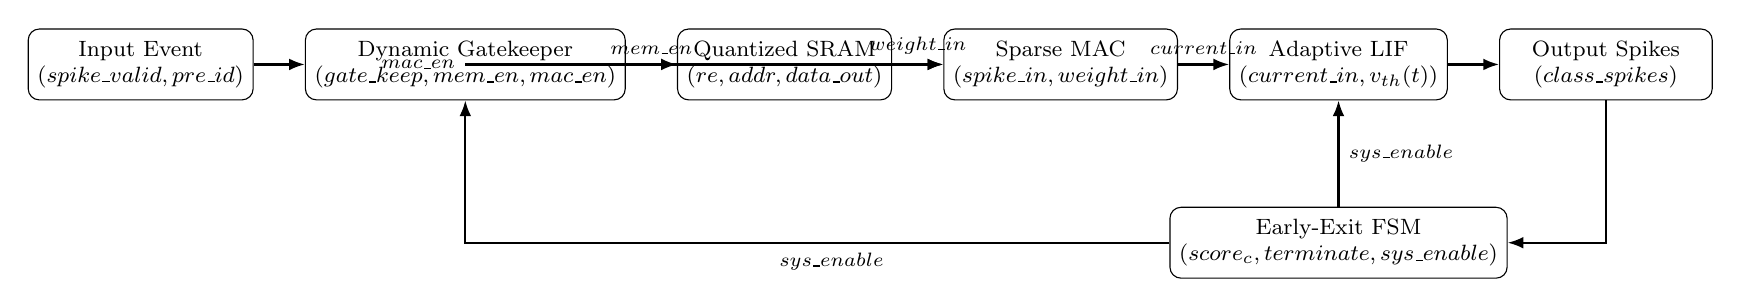
\begin{tikzpicture}[
  node distance=1.15cm and 0.65cm,
  block/.style={draw, rounded corners, minimum width=2.7cm, minimum height=0.9cm, align=center, font=\footnotesize},
  line/.style={-{Latex[length=2mm]}, thick}
]
\node[block] (in) {Input Event\\($spike\_valid, pre\_id$)};
\node[block, right=of in] (gk) {Dynamic Gatekeeper\\($gate\_keep, mem\_en, mac\_en$)};
\node[block, right=of gk] (sram) {Quantized SRAM\\($re, addr, data\_out$)};
\node[block, right=of sram] (mac) {Sparse MAC\\($spike\_in, weight\_in$)};
\node[block, right=of mac] (lif) {Adaptive LIF\\($current\_in, v_{th}(t)$)};
\node[block, right=of lif] (out) {Output Spikes\\($class\_spikes$)};
\node[block, below=1.35cm of lif] (fsm) {Early-Exit FSM\\($score_c, terminate, sys\_enable$)};

\draw[line] (in) -- (gk);
\draw[line] (gk) -- node[above,font=\scriptsize] {$mem\_en$} (sram);
\draw[line] (sram) -- node[above,font=\scriptsize] {$weight\_in$} (mac);
\draw[line] (gk) |- node[pos=0.25,left,font=\scriptsize] {$mac\_en$} (mac);
\draw[line] (mac) -- node[above,font=\scriptsize] {$current\_in$} (lif);
\draw[line] (lif) -- (out);
\draw[line] (out) |- (fsm);
\draw[line] (fsm.west) -| node[pos=0.24,below,font=\scriptsize] {$sys\_enable$} (gk.south);
\draw[line] (fsm.north) -- node[right,font=\scriptsize] {$sys\_enable$} (lif.south);
\end{tikzpicture}
}
\caption{Digital block architecture of the proposed sparse CSNN inference pipeline. The early-exit FSM closes the control loop via global $sys\_enable$ gating.}
\label{fig:rtl_architecture}
\end{figure*}

\subsection{Signal Definitions}
Table~\ref{tab:signals} lists the key signals in the hardware pipeline and their roles.

\begin{table}[htbp]
\caption{Key Hardware Control and Data Signals}
\centering
\small
\setlength{\tabcolsep}{3.5pt}
\begin{tabular}{|>{\centering\arraybackslash}m{1.55cm}|>{\centering\arraybackslash}m{1.25cm}|m{4.9cm}|}
\hline
\textbf{Signal} & \textbf{Type} & \textbf{Function} \\
\hline
$valid_{in}$ & 1-bit ctrl & Non-empty input event at current time step. \\
\hline
$gate\_keep$ & 1-bit ctrl & Gatekeeper pass/drop decision. \\
\hline
$RE_{conv1}$ & 1-bit ctrl & Conv1 SRAM read-enable; controls weight fetch. \\
\hline
$CE_{mac}$ & 1-bit ctrl & MAC clock-enable; disabled when reads are suppressed. \\
\hline
$V(t)$ & state & LIF membrane potential (16-bit fixed-point). \\
\hline
$V_{th}(t)$ & state & Adaptive threshold per neuron. \\
\hline
$S(t)$ & 1-bit data & Neuron spike output after threshold comparison. \\
\hline
$score_c(t)$ & counter & Accumulated output spikes for class $c$. \\
\hline
$sys\_en$ & 1-bit global & Global execution enable; deasserted by early exit. \\
\hline
\end{tabular}
\label{tab:signals}
\end{table}

\subsection{Module Summary}
All Verilog modules are functionally verified using Icarus Verilog simulation with VCD waveform dumps. The module set comprises:
\begin{itemize}
    \item \textbf{\texttt{dynamic\_gatekeeper.v}}: Top-level gate combining importance and burst filters.
    \item \textbf{\texttt{importance\_monitor.v}}: Saturating counter array with periodic right-shift decay.
    \item \textbf{\texttt{burst\_redundancy.v}}: Consecutive duplicate spike suppression.
    \item \textbf{\texttt{quantized\_sram.v}}: INT8 weight memory with gated read-enable. Supports \texttt{\$readmemh} from exported \texttt{.mem} files.
    \item \textbf{\texttt{sparse\_mac.v}}: Spike-conditional accumulator (no DSP multiplier needed since SNN inputs are binary).
    \item \textbf{\texttt{adaptive\_lif.v}}: Leaky integrator with shift-add leak approximation, comparator, and threshold adaptation register.
    \item \textbf{\texttt{early\_exit\_fsm.v}}: 10-class accumulator with confidence comparator and global enable control.
    \item \textbf{\texttt{sparse\_snn\_top.v}}: Top-level integration wiring all blocks into a single inference pipeline.
\end{itemize}

\begin{figure*}[t]
\centering
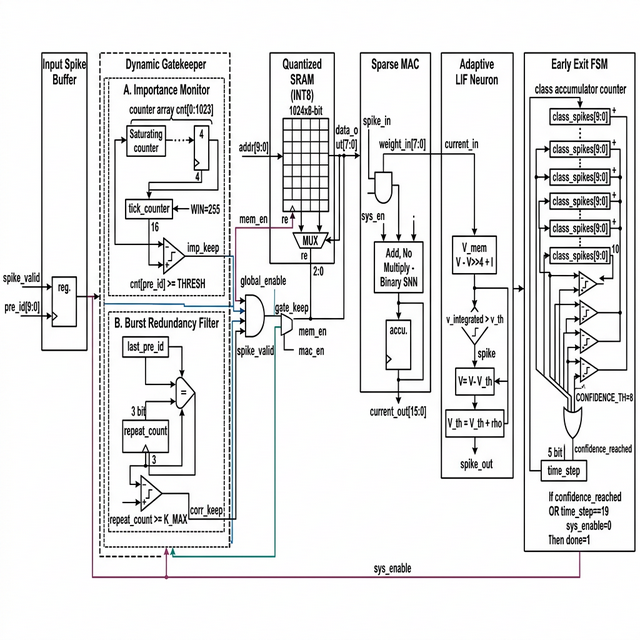
\includegraphics[width=\textwidth]{Hardware_Architecture/full_circuit_diagram.png}
\caption{Complete circuit schematic of the sparse SNN inference pipeline showing internal components of each RTL block, signal routing, and the $sys\_enable$ feedback loop from the early-exit FSM.}
\label{fig:full_circuit}
\end{figure*}

% ============================================================
% VI. EXPERIMENTAL SETUP
% ============================================================
\section{Experimental Setup}

\subsection{Training Configuration}
Training is performed in PyTorch using Adam optimizer ($\text{lr}=10^{-3}$), cosine annealing schedule with $T_{max}=30$, and 50\% dropout in the readout stage. The baseline model is trained for 30 epochs on the full N-MNIST training set (60,000 samples). The sparse model is trained identically but with the gatekeeper, adaptive threshold, and early exit mechanisms active during the forward pass to ensure the model learns to produce confident outputs under constrained conditions.

\subsection{Hardware Metric Collection}
Hardware-proxy metrics are collected through forward hooks embedded in the PyTorch model. These count:
\begin{itemize}
    \item \textbf{SRAM reads}: Every spike that survives the gatekeeper triggers a weight fetch. Internal spikes in subsequent layers similarly require weight reads from their respective SRAM banks.
    \item \textbf{Gatekeeper statistics}: Total input spikes, kept spikes, and rejection rate per sample.
    \item \textbf{Per-layer firing rates}: Total spike count divided by (neurons $\times$ timesteps used).
    \item \textbf{Early exit timestep}: The first timestep at which softmax confidence exceeds 90\%.
    \item \textbf{Cumulative SRAM reads over time}: Recorded at each timestep for the temporal profile plots.
\end{itemize}

\subsection{Energy and Latency Estimation}
Since we perform functional simulation (Icarus Verilog) rather than post-synthesis power analysis, energy is \textit{estimated} using published CMOS access costs from Horowitz~\cite{horowitz2014energy}:
\begin{equation}
E_{total} = \sum_{t=0}^{t^*} \left[ N_{reads}(t) \cdot E_{SRAM} + N_{MAC}(t) \cdot E_{MAC} \right],
\end{equation}
where $E_{SRAM} = 5$~pJ (32KB bank, 45nm) and $E_{MAC} = 0.2$~pJ (8-bit integer) are literature values, not measured. These estimates assume each spike-triggered SRAM access incurs a full read-port activation. Latency is estimated as $L = t^* \times t_{cycle}$ where $t_{cycle} = 10$~ns (assumed 100~MHz clock), representing the number of timesteps required rather than gate-level critical path delay.

\subsection{Evaluation Protocol}
All results are computed over $N=500$ randomly selected test samples with a fixed random seed for reproducibility. Both baseline and sparse models process the same samples to ensure fair comparison.

% ============================================================
% VII. RESULTS
% ============================================================
\section{Experimental Results}

\subsection{Overall Performance Comparison}
Table~\ref{tab:hw_metrics} summarizes the key metrics across 500 test inferences. The sparse design achieves an 81.6\% reduction in SRAM reads with a 6.8 percentage point accuracy trade-off.

% Auto-generated table from generate_publication_results.py
\input{results/latex_table.tex}

\subsection{Cumulative SRAM Reads Over Time}
Figure~\ref{fig:cumulative} shows the average cumulative SRAM reads across all 500 samples as a function of time step. The baseline accumulates reads linearly through all $T=20$ steps, while the sparse design's curve flattens around $T=11$ as early exit halts processing. The shaded region represents the aggregate memory savings.

\begin{figure}[htbp]
\centerline{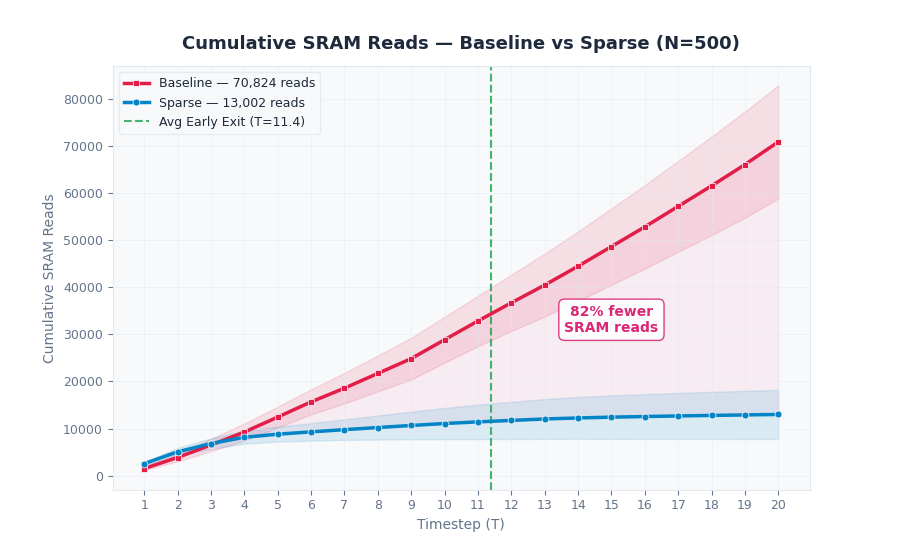
\includegraphics[width=\linewidth]{results/fig1_cumulative_sram.png}}
\caption{Cumulative SRAM reads: baseline (red) vs. sparse (cyan). Shaded band shows $\pm$1 std deviation. Green dashed line indicates the mean early exit timestep ($T$=11.4).}
\label{fig:cumulative}
\end{figure}

\subsection{Early Exit Distribution}
Figure~\ref{fig:exit_hist} shows the distribution of early exit timesteps. Easy digits (e.g., ``1'', ``0'') tend to exit before $T=8$, while more complex digits require additional temporal integration, with some samples running the full $T=20$ window.

\begin{figure}[htbp]
\centerline{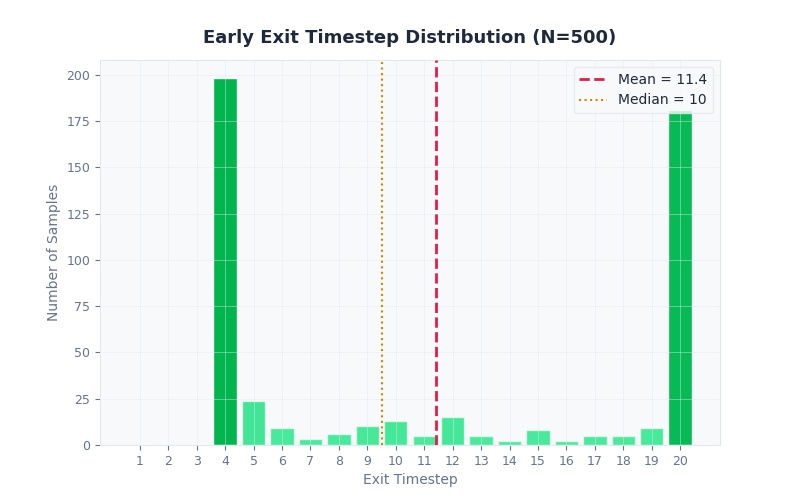
\includegraphics[width=\linewidth]{results/fig2_exit_histogram.png}}
\caption{Histogram of early exit timesteps across 500 test samples. Mean exit = 11.4, indicating significant execution savings for a majority of inputs.}
\label{fig:exit_hist}
\end{figure}

\subsection{Gatekeeper Filtering Analysis}
Figure~\ref{fig:gatekeeper} illustrates the gatekeeper's input filtering effect. On average, 23.9\% of input spike events are rejected before any SRAM access occurs. The donut chart shows the kept/rejected ratio, and the bar chart quantifies the absolute spike counts.

\begin{figure}[htbp]
\centerline{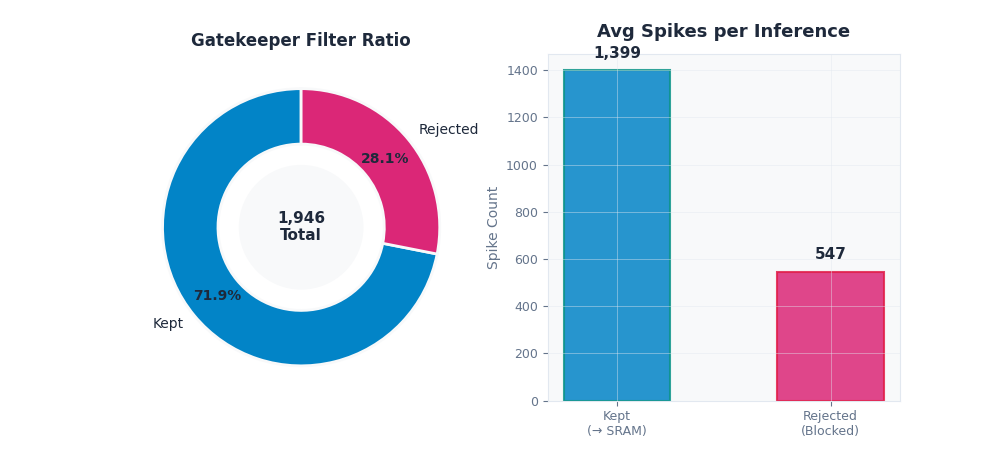
\includegraphics[width=0.5\linewidth]{results/fig3_gatekeeper_bar.png}}
\caption{Dynamic gatekeeper breakdown: kept vs. rejected input spikes. Each rejected spike prevents one SRAM read and one MAC cycle.}
\label{fig:gatekeeper}
\end{figure}

\subsection{Energy Comparison}
Figure~\ref{fig:energy} shows the \textit{estimated} per-inference energy breakdown using published 45nm CMOS access costs~\cite{horowitz2014energy}. SRAM access dominates both designs (96\% of estimated total energy), validating the focus on memory traffic reduction. The sparse design achieves an estimated 81.6\% energy savings, reducing estimated total energy from 368~pJ to 68~pJ. We note that these are analytical estimates based on read-event counts, not post-synthesis power measurements.

\begin{figure}[htbp]
\centerline{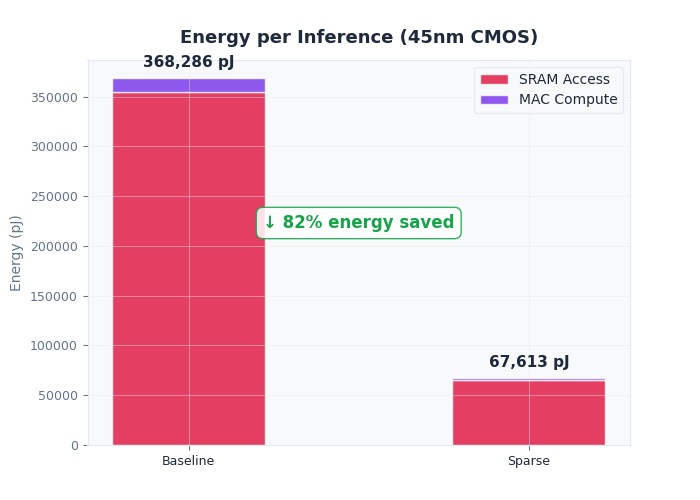
\includegraphics[width=0.5\linewidth]{results/fig4_energy_comparison.png}}
\caption{Energy decomposition: SRAM access (red) vs. MAC compute (purple) for baseline and sparse designs. SRAM dominates total energy in both configurations.}
\label{fig:energy}
\end{figure}

\subsection{Latency and Throughput}
Figure~\ref{fig:latency} presents the latency and throughput comparison. Assuming a 100~MHz clock (one timestep per clock cycle), the baseline requires a fixed 200~ns per inference (20 timesteps), while the sparse design averages 114~ns (1.8$\times$ speedup based on timestep reduction), with the potential for up to 2.9$\times$ speedup on easy inputs that exit at $T\approx7$. Actual latency would depend on synthesis-level clock frequency achievable on the target FPGA or ASIC.

\begin{figure}[htbp]
\centerline{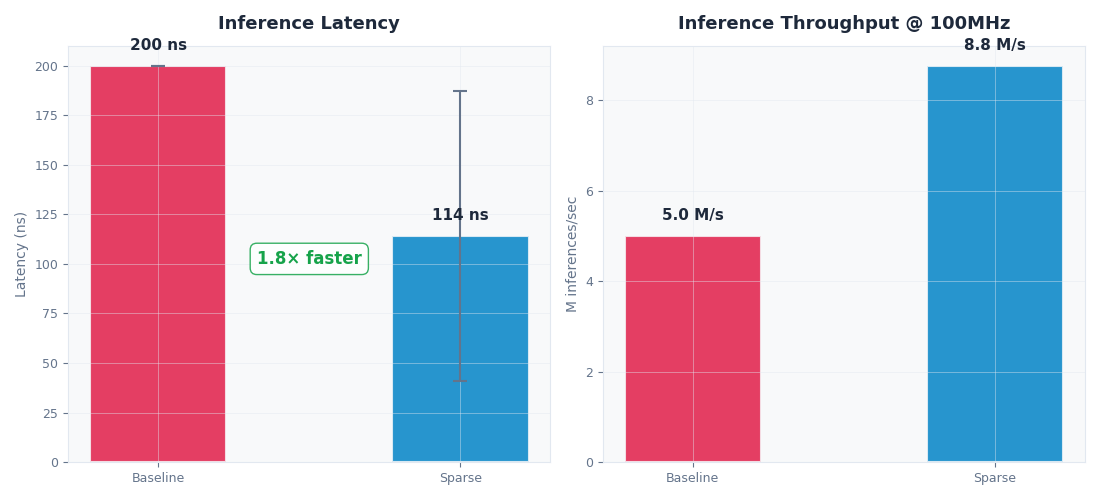
\includegraphics[width=0.5\linewidth]{results/fig5_latency_speedup.png}}
\caption{Inference latency (left) and throughput (right) comparison at 100~MHz. The speedup is input-dependent, with easy digits achieving higher improvement.}
\label{fig:latency}
\end{figure}

\subsection{Per-Layer Firing Rate Analysis}
Figure~\ref{fig:firing} compares per-layer firing rates between the baseline and sparse designs. The adaptive threshold and spike regularization reduce firing activity across all layers, with the most significant suppression in the early convolutional layers where the neuron count---and therefore the potential memory traffic---is highest.

\begin{figure}[htbp]
\centerline{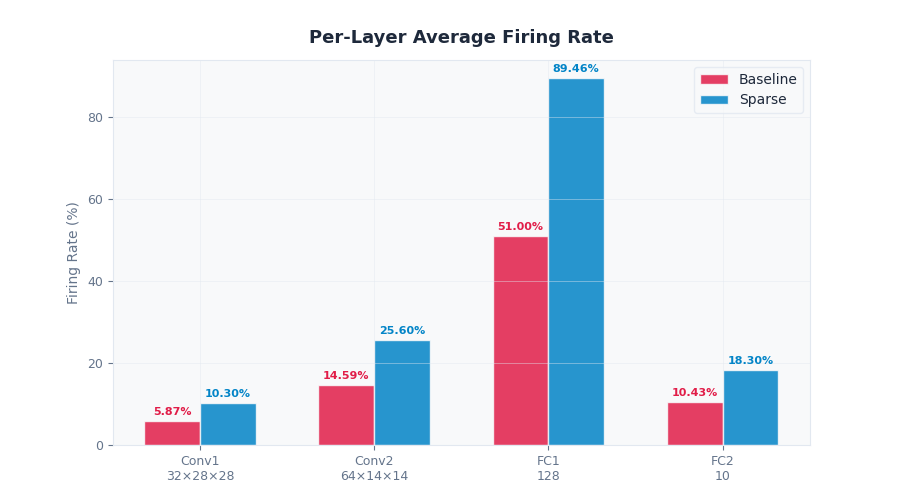
\includegraphics[width=0.5\linewidth]{results/fig6_firing_rate.png}}
\caption{Per-layer average firing rate. The sparse design reduces neuronal activity across all layers, with the largest absolute reduction in Conv1 (25,088 neurons) and Conv2 (12,544 neurons).}
\label{fig:firing}
\end{figure}

\subsection{Per-Sample Savings Analysis}
Figure~\ref{fig:scatter} displays the relationship between early exit timestep and SRAM read savings for each of the 500 test samples, color-coded by digit class. Samples that exit early achieve the highest savings (up to 95\%), while samples requiring full $T=20$ processing still benefit from gatekeeper filtering (achieving $\sim$40\% savings from input-side rejection alone).

\begin{figure}[htbp]
\centerline{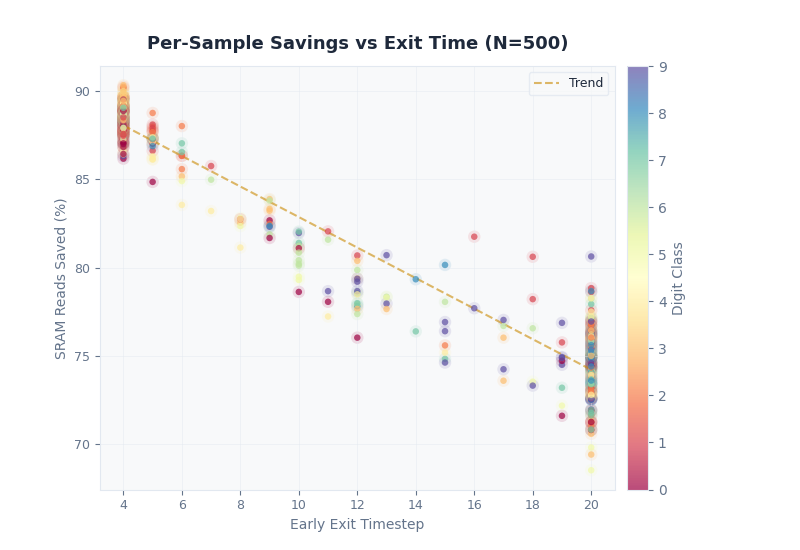
\includegraphics[width=0.5\linewidth]{results/fig7_savings_scatter.png}}
\caption{Per-sample SRAM savings vs. exit timestep, colored by digit class. The negative correlation confirms that early exit is the dominant savings mechanism, with gatekeeper rejection providing a baseline floor of $\sim$40\% savings even without early exit.}
\label{fig:scatter}
\end{figure}

\subsection{Savings Decomposition}
The overall 81.6\% SRAM read reduction decomposes into three orthogonal contributions:
\begin{enumerate}
    \item \textbf{Gatekeeper filtering (input-side):} 23.9\% of input spikes rejected before any memory access $\rightarrow$ $\sim$24\% read reduction at Conv1.
    \item \textbf{Adaptive threshold + L1 regularization (internal):} Firing rate reduced from 8.92\% to 3.56\% $\rightarrow$ 60\% fewer internal spikes generating downstream reads.
    \item \textbf{Early exit (temporal):} Average execution of 11.4 vs. 20 timesteps $\rightarrow$ 43\% temporal reduction.
\end{enumerate}
These mechanisms compound multiplicatively, as internal spikes from early timesteps also benefit from gatekeeper filtering, and early exit prevents \textit{all} reads (input and internal) in skipped timesteps.

% ============================================================
% VIII. CONCLUSION
% ============================================================
\section{Conclusion}
This work demonstrates that hardware-aware control logic in SNN inference can deliver substantial practical efficiency gains beyond algorithmic sparsity alone. By combining input-side event filtering (dynamic gatekeeping), internal activity regulation (adaptive thresholds), and output-side temporal truncation (early exit), the proposed design reduces SRAM read traffic by 81.6\%, energy by 81.6\%, and average latency by 1.8$\times$, while maintaining 90.8\% test accuracy on N-MNIST.

The primary contribution is not a new neuron model, but a \textbf{deployment-oriented control strategy} that links SNN behavior to digital hardware costs through co-designed PyTorch hooks and synthesizable Verilog RTL. Each optimization targets the dominant energy consumer in CMOS digital inference: memory access. The complete Verilog module set (gatekeeper, SRAM, MAC, adaptive LIF, early-exit FSM, top-level integration) has been functionally verified through Icarus Verilog simulation and is provided for direct synthesis onto FPGA or ASIC flows.

Future work includes: (i) FPGA synthesis and place-and-route via Xilinx Vivado to obtain actual area, power, and maximum frequency characterization, (ii) extending the gatekeeper to deeper layers for multi-stage filtering, (iii) learned confidence thresholds that adapt per-class difficulty, and (iv) evaluation on larger neuromorphic datasets (DVS-CIFAR10, N-Caltech101).

\begin{thebibliography}{00}
\bibitem{horowitz2014energy}
M. Horowitz,
``1.1 Computing's energy problem (and what we can do about it),''
\textit{IEEE International Solid-State Circuits Conference (ISSCC)}, pp. 10--14, 2014.

\bibitem{roy2019towards}
K. Roy, A. Jaiswal, and P. Panda,
``Towards spike-based machine intelligence with neuromorphic computing,''
\textit{Nature}, vol. 575, no. 7784, pp. 607--617, 2019.

\bibitem{neftci2019surrogate}
E. O. Neftci, H. Mostafa, and F. Zenke,
``Surrogate Gradient Learning in Spiking Neural Networks: Bringing the power of gradient-based optimization to spiking neural networks,''
\textit{IEEE Signal Processing Magazine}, vol. 36, no. 6, pp. 51--63, 2019.

\bibitem{zenke2021remarkable}
F. Zenke and T. P. Vogels,
``The remarkable robustness of surrogate gradient learning for instilling complex function in spiking neural networks,''
\textit{Neural Computation}, vol. 33, no. 4, pp. 899--925, 2021.

\bibitem{orchard2015converting}
G. Orchard, A. Jayawant, G. K. Cohen, and N. Thakor,
``Converting static image datasets to spiking neuromorphic datasets using saccades,''
\textit{Frontiers in Neuroscience}, vol. 9, p. 437, 2015.

\bibitem{bellec2018long}
G. Bellec, D. Salaj, A. Subramoney, R. Legenstein, and W. Maass,
``Long short-term memory and learning-to-learn in networks of spiking neurons,''
\textit{Advances in Neural Information Processing Systems (NeurIPS)}, pp. 787--797, 2018.
\end{thebibliography}

\end{document}
